\section{Preliminary Results}

%Intro describing the project and add link to GitHub!

The most updated version of COATi can be found as an open source project on
\href{https://www.github.com/jgarciamesa/coati}{GitHub}.
Written in C++ 17, COATi can be build using the open source software Meson.
Once compiled, it can be run from the command line using the syntax
\texttt{coati command arguments [options]}

The software development cycle follows best practices including continuous
integration, unit testing with doctest, linting and formatting according to the
Google C++ stylesheet with clang.
Results from continuous integration together with test coverage are displayed
on the GitHub repository.

Currently, COATi includes a functional version of \texttt{coati alignpair}, a
pairwise aligner that offers different substitution models and can find an
an optimal alignment given a low and a high-quality sequence.
The software package also includes a utility command \verb|coati format| that is
able to convert between fasta and phylip formatted files as well as extract
specific sequences from a multi-sequence input.
In addition, \texttt{coati msa}, under development, produces an initial multiple
sequence alignment given a phylogenetic tree in newick format.

To illustrate the obstacles with current aligners and to showcase the
performance of COATi, I have simulated pairwise alignments with empirical gaps
patterns and evaluated the accuracy of popular cutting edge aligners
%BAli-Phy \parencite{suchard_baliphy_2006},
Clustal$\Omega$ \parencite{clustal_omega_sievers_2011}, MACSE
\parencite{ranwez_macse_2011}, MAFFT \parencite{mafft_katoh_2002}, and PRANK
\parencite{prank_loytynoja_2014} together with COATi.

I downloaded 4000 human genes and their gorilla homologous pairs from the
ENSEMBL database \parencite{ensembl_hubbard_2002} and aligned them using all
five aligners.
From those, 1660 alignments contained gaps identified by at least one method.
Gap patterns extracted from all five methods were randomly introduced into the
other 2340 initially ungapped sequence pairs to generate the `true alignments'
Alignment accuracy was measured using the distance metric $d_{seq}$
\parencite{metrics_blackburne_whelan_2011} between simulated and inferred
alignments.
In addition, accuracy of positive and negative selection was calculated % using
% the $F_1$ score. explain why the F1 score was used?

% Software comparison table
\begin{table}[h!]
\centering
    \frame{% \begin{table}[h!]
% \begin{adjustbox}{width=\columnwidth,center}
\begingroup\centering
\begin{tabular}{r|cccccc}
      & \textbf{COATi} & \textbf{PRANK} & \textbf{MAFFT} & \textbf{CLUSTAL $\Omega$} & \textbf{MACSE} & \textbf{BAli-Phy} \\
\hline
Avg alignment error ($d_{seq}$) & 0.00055 & 0.00119 & 0.00373 & 0.00890 & 0.01547 & 0.00132\\
Perfect alignments & 871 & 579 & 747 & 370 & 532 & 588\\
% \hline
$k_a$ root mean-squared error & 0.00051 & 0.01059 & 0.05000 & 0.05621 & 0.03343 & NA\\
$k_s$ root mean-squared error & 0.00132 & 0.02564 & 0.05198 & 0.07371 & 0.06636 & NA\\
Positive selection F1 score & 98.6\pct & 16.3\pct & 71.3\pct & 61.7\pct & 66.1\pct & NA\\
Negative selection F1 score & 99.9\pct & 92.5\pct & 97.2\pct & 96.5\pct & 97.4\pct & NA
\end{tabular}
\par\endgroup
% \end{adjustbox}
% \end{table}
}
	\caption{Accuracy of COATi, PRANK, MAFFT, CLUSTAL$\Omega$, and MACSE,
            on 2340 simulated sequence pairs. Perfect alignments have
            ($d_{seq}=0$), best alignments have lowest $d_{seq}$, and imperfect
            alignments have $d_{seq}>0$ when at least one aligner found a perfect
            alignment.}
	\label{table:comp}
\end{table}

\textbf{Results.}
COATi was significantly more accurate (lower $d_{seq}$) than other aligners, all
p-values were equal (MAFFT) or less than $1.714$x$10^{-8}$ according to the one-tailed
Wilcoxon signed rank test.
In addition, COATi produced more perfect alignments, less imperfect alignments,
and had a higher positive and negative selection accuracy
(Table \ref{table:comp}).

MACSE was the only software to model frameshifts and out-of-phase gaps.
Despite claiming a hybrid method that combines information from both DNA and
amino acid levels, the implementation of MACSE is based solely on amino acid
translation and scored using the popular BLOSUM62 \parencite{henikoff1992amino}
matrix, for simplicity and speed reasons, as reported in
\cite{ranwez_macse_2011}.

Among the remaining aligners, MAFFT was run with a DNA model, CLUSTAL$\Omega$
performed a common strategy of aligning via amino acid translation, while PRANK
was the only aligner with a codon model available.
However, when using the codon model, PRANK replaces any unknown codons with
`NNN', modifying the original sequences and losing information.

% comparison of FST vs DP

% despite having an C++ FST library the runtime and memory requirements are
%  limiting/excessive
To showcase the limitations of pairwise alignment using FSTs I benchmarked
the FST version and the dynamic programming counterpart.
Despite the existence of efficient C++ FST libraries and the usage of known
optimization techniques, the runtime and memory requirements are impractical
for sequences longer than a few hundred bases.
% with the conversion/adaptation of the model to a DP format runtime and memory
%  become feasible
Fortunately, the dynamic programming adaptation of COATi's model
reduces costs significantly to levels similar to current aligners
(Fig. \ref{fig:benchmark}).

% \begin{wrapfigure}{r}{0.65\textwidth}
% % \begin{framed}
%     \includegraphics[scale=0.5]{figures/fst_vs_dp.pdf}
%     \caption{Caption.}
%     \label{fig:fst_vs_dp}
% % \end{framed}
% \end{wrapfigure}

% comparison of COATi vs other aligners - runtime

% continuing? from previous paragraph
%  coati is similar/in line with other alignments, thus making it a valid
%  solution (word better).
% maybe intro with something like, being accurate is not enough if the runtime
%  is too much of a limiting factor.

\begin{figure}[h!]
% \begin{framed}
    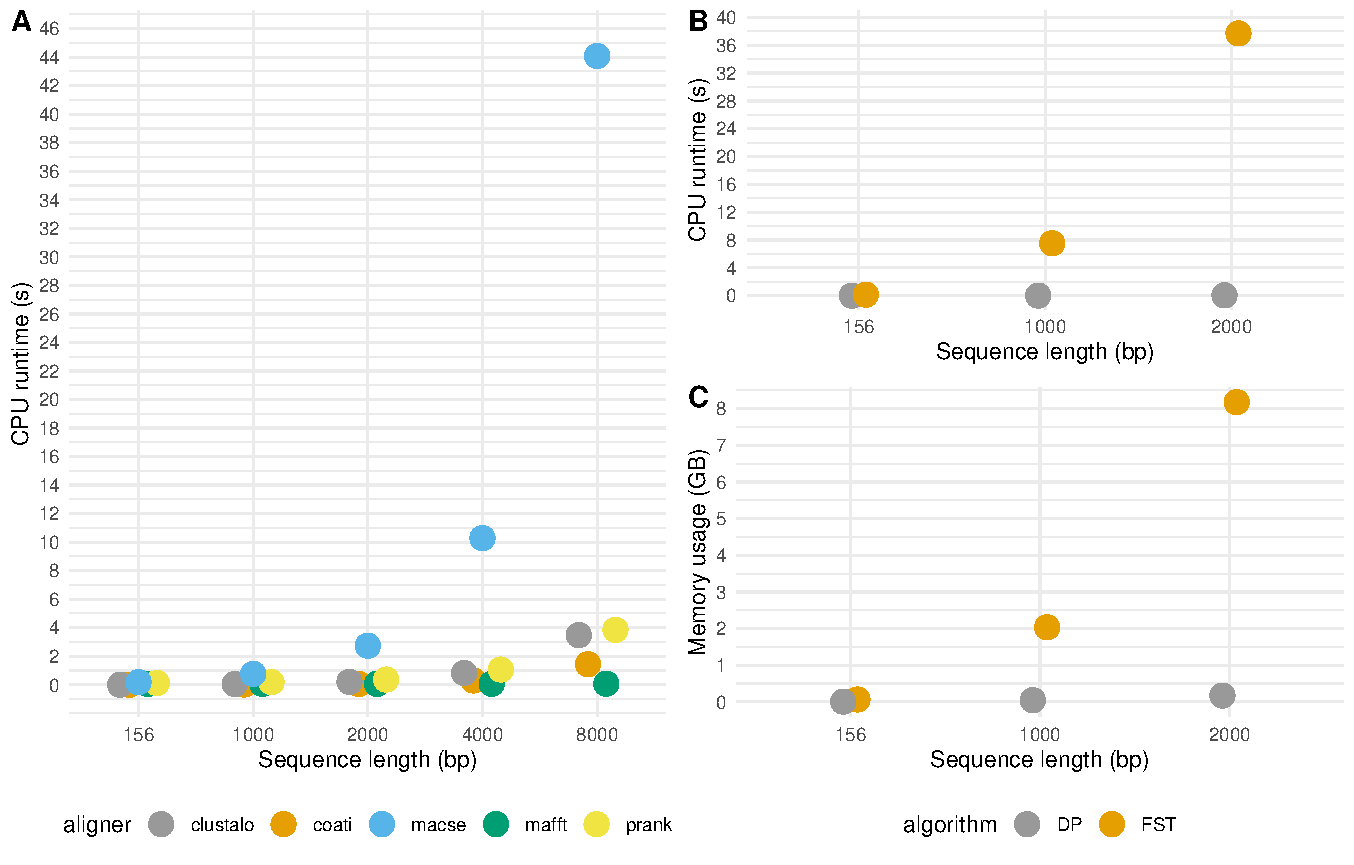
\includegraphics[scale=0.8]{figures/benchmark_fst_dp_alns.pdf}
    \caption{Runtime benchmark in seconds of CLUSTAL$\Omega$, COATi, MACSE,
    MAFFT, and PRANK aligning pairwise sequences of different lengths (A).
    Runtime (B) and memory usage (C) of COATi when aligning pairwise sequences
    of different lengths when using FSTs and a dynamic programming approach.}
    \label{fig:benchmark}
% \end{framed}
\end{figure}
